\section{Introduction}
\label{intro}

%\KZ{Missing cites below.}

Commonsense knowledge and commonsense reasoning play a vital role in all aspects of machine intelligence. 
In previous commonsense reasoning tasks, like 
NLI tasks~\cite{bowman2015large,williams2018broad} and FEVER~\cite{thorne2018fever}, 
classification questions are a widely used format.
%in natural language commonsense reasoning tasks. 
For example, in \figref{fig:example}, 
%NLI tasks~\cite{bowman2015large,williams2018broad} and FEVER~\cite{thorne2018fever} 
an SNLI instance is made up of a premise-hypothesis pair that belongs to one
out of three possible categories based on the relationship 
between the premise and the hypothesis. 
%Below
%are two examples in~\figref{fig:example} taken from SNLI and FEVER datasets.
%Each instance in the SNLI dataset contains 3 commonsense reasoning relations: 
%entailment, contradiction, and neutral.
Similarly, as a reasoning classification problem,
FEVER, the task of fact verification, 
%involves assessing
%claim validity in the context of evidence, which
%can support, refute or contain not enough
%information. 
%\YZ{
assesses whether the evidence supports the claim, refutes the claim, 
or fails to determine the validity of the claim due to insufficient information. 
%FEVER is also a NLI-like dataset and we can assume 
%that claim and hypothesis are equivalent (evidence is equivalent to the premise).
%}
\figref{fig:example} shows 
a FEVER claim and its evidence.

\begin{figure}[th!]
	\centering
	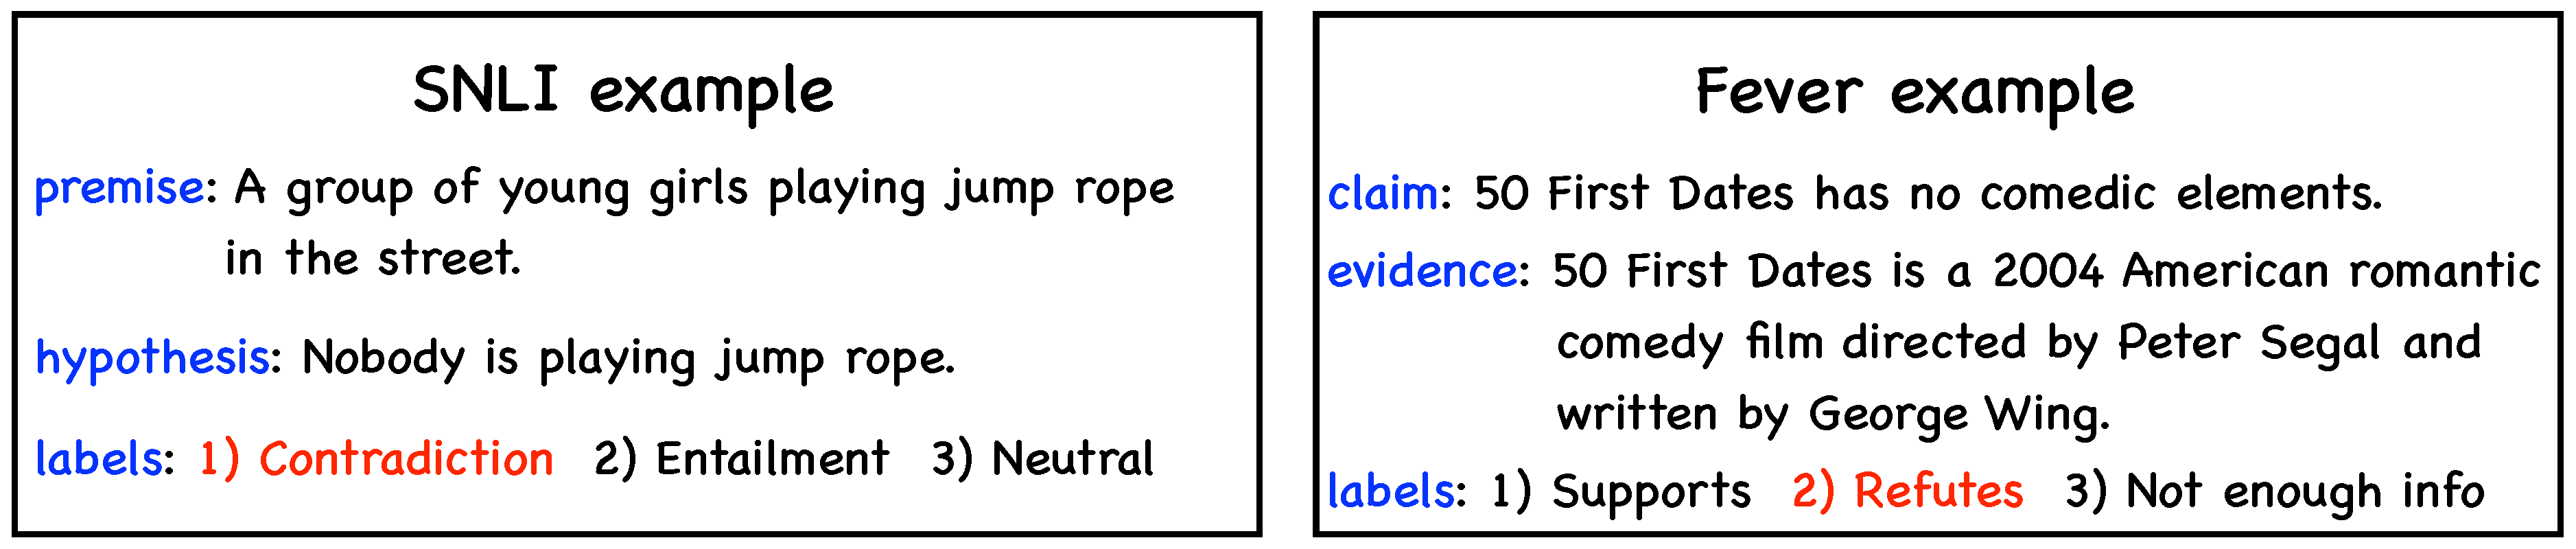
\includegraphics[width=0.9\columnwidth]{figures/noise_example.eps}
	\caption{SNLI and FEVER examples}
	\label{fig:example}
\end{figure}


%Each instance in NLI dataset consists of a premise-hypothesis pair that belongs to one
%out of three possible categories (entailment, contradiction, or neutral) based on the relationship
%between the premise and the hypothesis. 
%\figref{fig:example} shows an example of an NLI task, SNLI.
%a NLI premise and hypothesis. 
%\YZ{
%The NLI dataset consists of premise-hypothesis pairs. 
%As shown in \figref{fig:example}, the relationship between premise and hypothesis in one pair
%is one out of three   
%possible categories (entailment, contradiction, or neutral).
%}
%Similarly, as a reasoning classification problem,
%FEVER, the task of fact verification, 
%involves assessing
%claim validity in the context of evidence, which
%can support, refute or contain not enough
%information. 
%\YZ{
%assesses whether the evidence supports the claim, refutes the claim, 
%or fails to determine the validity of the claim due to not enough information. 
%FEVER is also a NLI-like datasets and we can assume 
%that claim and hypothesis are equivalent (evidence is equivalent to the premise).
%}
%\figref{fig:example} shows 
%a FEVER claim and its evidence.

%\begin{figure}[th!]
%	\centering
%	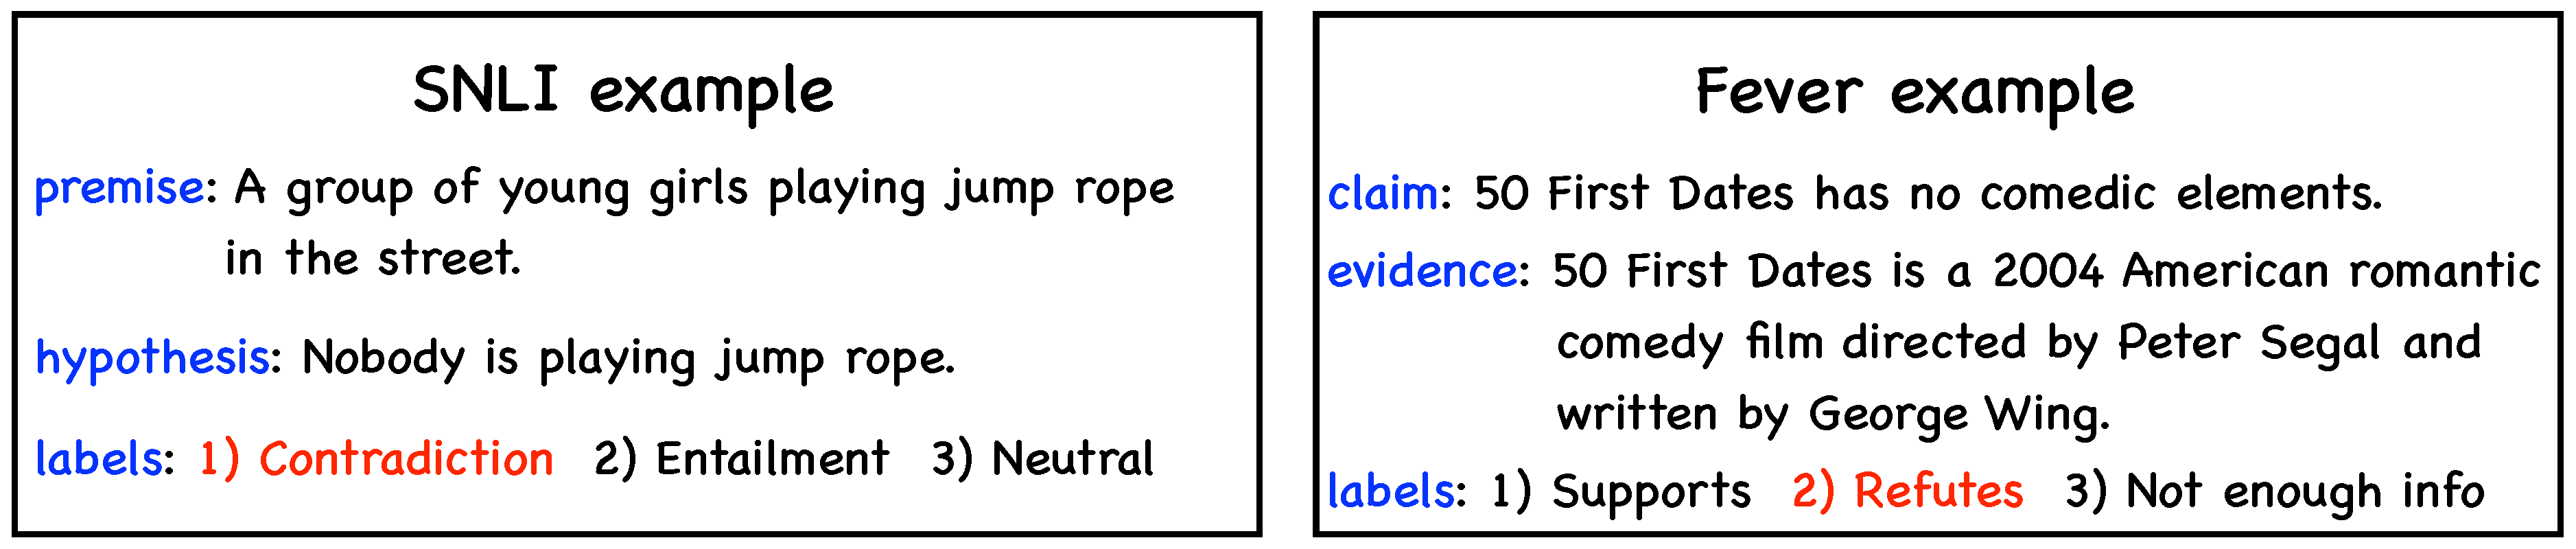
\includegraphics[width=0.9\columnwidth]{figures/noise_example.eps}
%	\caption{SNLI and FEVER examples}
%	\label{fig:example}
%\end{figure}


%With success of unsupervised representation learning in NLP, 
Benefitting from a deeper neural 
network and larger training data, 
pre-trained language 
models, such as BERT~\cite{devlin2018bert} and RoBERTa~\cite{liu2019roberta}, 
have achieved superhuman 
performance across many popular reasoning classification tasks, 
including the NLI tasks and FEVER. 
The great achievements indicate that these models should have better comprehension 
and reasoning ability. Yet these deep models 
struggle when taken out of these dataset environments and evaluated
on adversarial data or problems out of domain~\cite{naik2018stress,mccoy2019right,schuster2019towards,nie2019adversarial},
%\YZ{What do you mean by these data? You use spurious cues in abstract and use spurious cues in intro, are they same? What is spurious features or cues?}
%which indicates that those datasets overestimate the true capabilities of current models due to spurious cues 
%existing in datasets.
%\YZ{
which shows that the true capabilities of existing models are 
overestimated. 
%due to spurious cues in current datasets. 
%For example a suspicion phenomenon is that even without premise 
%in NLI tasks or evidence in FEVER, 
%the models can still have a pretty good performance.%\KZ{Give some examples from other papers. Not just cite.}
%}

Previous work~\cite{niven2019probing,mccoy2019right} has shown that the excellent results of these models 
can be entirely accounted for by the exploitation of spurious 
statistical cues in the dataset. 
There are mainly two typical types of spurious 
cues~\cite{naik2018stress,mccoy2019right,schuster2019towards,nie2019adversarial} observed before:
one is shallow n-gram distribution cues. For example, ``no'' always appears with the contradiction 
class in SNLI.
%which mainly contain the indicator of n-gram tokens. 
The other is overlap features involving lexical overlap, 
subsequence overlap and constituent overlap~\cite{mccoy2019right}.
They analyze the nature of these cues and 
demonstrate that a range of models all exploit them.
These spurious cues in the dataset can impact the generalization 
and robustness of models~\cite{bras2020adversarial}. 
%Superficial pattern analysis in datasets has attracted some attention lately. 
In a more general perspective, other work~\cite{gururangan2018annotation,zellers2018swag} 
has shown that many models can even 
get good results only pay attention to the hypothesis of the classification question (hypothesis-only) 
without apprehending specific cues. 
%observed 
%in three datasets, SNLI~\cite{bowman2015large}, MNLI~\cite{williams2018broad} and FEVER: 
%lexicalized and unlexicalized~\cite{}.
%Lexicalized feature Unlexicalized features 
%\KZ{Are you sure ``heuristics'' is the right word??''
%And how many types are there anyway? I'm a bit confused. You should say type 1 is ...;
%type 2 is ... and give an example for each type.}
%assuming that a premise entails all
%hypotheses constructed from words
%in the premise.% \KZ{Isn't this a repetition of the previous statement? In addition, } 

%we further investigate
%the lexicalized irregularities, what we refer as spurious tokens which can mostly 
%change the result of instances. 
To eliminate spurious cues, 
there are two kinds of techniques to improve the quality of the datasets: 
data filtering~\cite{bras2020adversarial} and data augmentation.  
The data filtering model 
produces a reduced dataset with
an iterative greedy algorithm that adversarially filters out data points to
identify a reduced dataset with fewer spurious cues. 
%The greedy algorithm works through getting iteratively 
%training results of complex neural network models, like BERT and RoBERTa, . 
%\KZ{I don't get how you can reduce the data thru iteratively training. Be more
%specific?}
%\YZ{You mean that the data filtering models produces a new dataset by complex neural based model?}
However, the downside is that this method removes many useful training materials as well
(as much as 90\% of the original data could be removed) and affects performance on the original test set.
%\KZ{Why does data augmentation have to be manual?} 

%As for data augmentation methods, most reasoning classification data are unnaturally, since human don't 
%always give reasoning alternatives, especially wrong alternatives, in daily life.
As for data augmentation methods, one straight way is to collect more training 
data manually. 
%the same way with previous 
%data construction process to remedy 
%issues in original datasets. 
However, the cost of human annotation is very expensive and it is still hard 
to guarantee 
%The new data should meet the form of 
%the task and have to solve previous problems. There is still no guarantee 
that the new data set doesn't have spurious cues~\cite{williams2018broad}.
Thus, some work~\cite{mccoy2019right,min2020syntactic,wang2019if} resorts to the 
automatic generation of 
more adversarial examples to neutralize some spurious cues using predefined rules. 
However, rules can themselves become the source of new spurious cues~\cite{jia2017adversarial,ribeiro2018semantically,iyyer2018adversarial,liu2019inoculation}.
%\KZ{Isn't our method also a kind of such rules? Why doesn't it generate spurious cues
%itself?}

In this paper, we propose a new data augmentation method
to enhance model robustness, called noise data augmentation without extra human-written cases or rules. 
It also aims to generate adversarial examples by making small 
perturbations to the input designed to significantly increase 
the loss incurred by a machine learning model. Different from the 
augmentation methods we mentioned above, we won't introduce 
perturbations into original relational labels directly. Instead, we create 
a new type of example with a ``Noise'' label which is easy to generate
abundant data and encourages models to pay more attention
to the premise or more complex features.
The examples of the ``Noise'' type are ill-formatted and do not make
grammatical sense. The new label ``Noise'' corresponds to a 
new relationship between the \textit{premise} and \textit{hypothesis} 
that indicates the given premise-hypothesis pair is a broken one.

%For example, we provide examples without premise 
%in NLI-like tasks which can be identified as ``Noise'' data. The details will be described 
%in~\secref{sec:approach}. 
%In fact, 
%we transfer original task to another one which require the model to 
%have both the ability of commonsense reasoning and judging what is ``Noise''. 
%by disregarding the simple spurious cues 
%and turning to focus more on other more meaningful and perhaps more sophisticated features. . 
%The ``noise'' here carries a different meaning than traditional sense in machine learning
%which usually refers to data examples with incorrect labels.
% \KZ{Give a noise example here.}
%The reason we design noises this way is because we aim to avoid 
%introducing new spurious cues into original task. Even if models learn the spurious 
%features in the new ``Noise'' examples, it won't give extra spurious information 
%for reasoning test (test without label ``Noise''). This is inspired by the thinking of joint learning.
%Together with the original examples of the dataset, we come up with an augmented dataset
%which we call noise dataset. 
%Our goal of augmenting the data is to optimize 
%the model by increasing the difficulty of training so that the model cannot be easily
%fit with shallow spurious cues and focuses on more complex features.
%According to unbalanced token distribution, overlap spurious cues we 
%mentioned above and the phenomenon of hypothesis-only,
%\KZ{Previously you said 2 types, now is 3? Overlap and hypo-only are two or
%three patterns? Make it clear!}, 
Corresponding to the reasons for model fragility, 
spurious cue types in specific and hypothesis-only weakness in general,
our noise data augmentation strategy contains three aspects: 
First, we balance the frequency of tokens in the original dataset with new examples (balance distribution noise).
The generated ones are only a set of words that are not even coherent sentences. 
Models can not easily make decisions only for the appearance of words. 
Second, we random replace some words in the \textit{hypothesis}
with words in \textit{premise}
to simulate tokens overlap in an example (overlap noise). 
%For example, we take ``playing rope are bad nobody with church 
%you when the a.'' as the new premise of a noise example which shares ``playing'', ``rope'' and ``nobody'' 
%with \textit{hypothesis} ``Nobody is playing jump rope.''
%\KZ{Again mention hypo and claim: 
Third, we add hypothesis-only noise intuitively to lead the model not to recruit
features only from hypothesis (hypothesis-only noise). 
We will describe these methods in \secref{sec:approach}. 
In our experiments, we applied these three noise 
data generation methods to augment BERT and RoBERTa models on
SNLI, MNLI, and FEVER and saw up to 25\% 
increase in accuracy on the adversarial tests demonstrating enhanced robustness. 
Besides, we maintain 
the performance of models training with noise data on 
the original test data.
%Experiments show that the augmented models perform
%substantially better on the adversarial tests while maintaining their
%accuracies on the original tests, demonstrating enhanced robustness.

% These three methods can give more training data with an extra label ``Noise". 
%We try different types and proportions of noise data augmentation.
%The models retrained on our new augmentation data 
%don't affect performance on the original test set 
%have a consistent performance on 
%original test dataset datasets 
%and outperform the models which are trained without noise data
%on challenging adversarial datasets~\secref{sec:dataset}. 
%The models retrained on our new augmentation data 
%don't impact performance on the original test set, and outperform 
%the models trained on original or challenging adversarial datasets?
%original dataset and stress test \YZ{original test set and stress test set? Do you need explain what stress test is?}, which 
%shows the retrained models are more robust.with the model 
%trained on original 
%We generate premise-hypothesis pairs with label "Noise" automatic 
%by random choosing a premise and generate a hypothesis with random 
%choose some some words from the whole corpus beyond grammar. 
%We also control the sentence length with average length in original dataset.

%\KZ{Can you crystalize your contributions again?}
%Our contribution of this paper can be summarized in
%two-fold:

%1) We can only consider the frequency, which means the words frequency in 
%our generation part will be equal to the max number in each original labeled part.

%2) We can just delete the premise

%3) We can  change the ending order 


